\documentclass[12pt]{article}
\usepackage[margin=1in]{geometry} 
\usepackage{graphicx}
\usepackage{amsmath,amsthm,amssymb}
\usepackage{hyperref}
\usepackage{mathrsfs}
\usepackage{xcolor}

\title{
    \textbf{MS5033} \\
    \textbf{Mesoscale Microstructure Modeling} \\ 
    \textbf{Report} \\
}

\author{
    \begin{tabular}{c}
        \textbf{Darpan Gaur} \\
        \textbf{CO21BTECH11004}print(f"Initialization completed")
    \end{tabular}
    \begin{tabular}{c}
        \textbf{Yoshita Kondapalli} \\
        \textbf{CO21BTECH11008}
    \end{tabular}
}

\date{}

\begin{document}
\maketitle

\hrulefill

\section*{Problem Statement}
In this project, we simulate the growth of a solid tumor using a Cahn–Hilliard-type convection-reaction-diffusion model. The goal is to capture the evolution of tumor volume fraction, nutrient concentration, and velocity fields in a confined domain over time. This type of modeling is useful for understanding tumor development, interactions with the microenvironment, and for testing hypothetical therapies. 

\section{Mathematical Model}
Governing equtaions are as follows:
\begin{equation}
    \frac{\partial \phi}{\partial t} = \textcolor{red}{\nabla \cdot \left( M(\phi) \nabla \mu \right)} + \textcolor{blue}{\bar{\rho}_S (P\sigma -A) h(\phi)} - \textcolor{green}{\nabla \nu \phi}
    \label{eq:phi}
\end{equation}
Equation \ref{eq:phi}, consists of three terms:
\begin{itemize}
    \item \textcolor{red}{Diffusion term}: Describes the diffusion of the tumor phase $\phi$.
    \item \textcolor{blue}{Source term}: Represents the growth of the tumor due to nutrient availability.
    \item \textcolor{green}{Chemotaxis term}: Represents the chemotactic response of the tumor to nutrient gradients.
\end{itemize}
\begin{equation}
    \mu = \frac{\beta}{\epsilon} \psi(\phi) - \beta \epsilon \Delta \phi - \chi_\phi \sigma
\end{equation} 
\begin{equation}
    \frac{\partial \sigma}{\partial t} = \nabla \cdot (n(\phi) (\chi_\sigma \nabla \sigma - \chi_\phi \nabla \phi)) - C \sigma h(\phi)
\end{equation}
\begin{equation}
    \nu = - K (\nabla P - \mu \nabla \phi - \chi_\phi \sigma \nabla \phi)
\end{equation}

\section*{Results}
\begin{itemize}
    \item Here $t=1$ signifies, 1000 timesteps, with stepsize of 0.001.
    \item $\chi$ is the chemotaxis parameter.
    \item $\sigma$ denotes the unspecified chemical species that serves as nutrients for tumor.
    \item $\phi$ phase variable denotes the tumor volume fraction.
\end{itemize}
\subsection*{$\sigma$ Evolution}
Figure \ref{fig:sigmaVsT_scatter_chi5} and \ref{fig:sigmaVsT_contour_chi5} show the evolution of $\sigma$ with time for $\chi_\phi=5$ by plotting the scatter and contour plots respectively. 

\begin{figure*}
    \centering
    \includegraphics[width=1.0\textwidth]{../sigmaVsT_scatter_chi5.png}
    \caption{Scatter plot of $\sigma$ with time evolution.}
    \label{fig:sigmaVsT_scatter_chi5}
\end{figure*}
\begin{figure*}
    \centering
    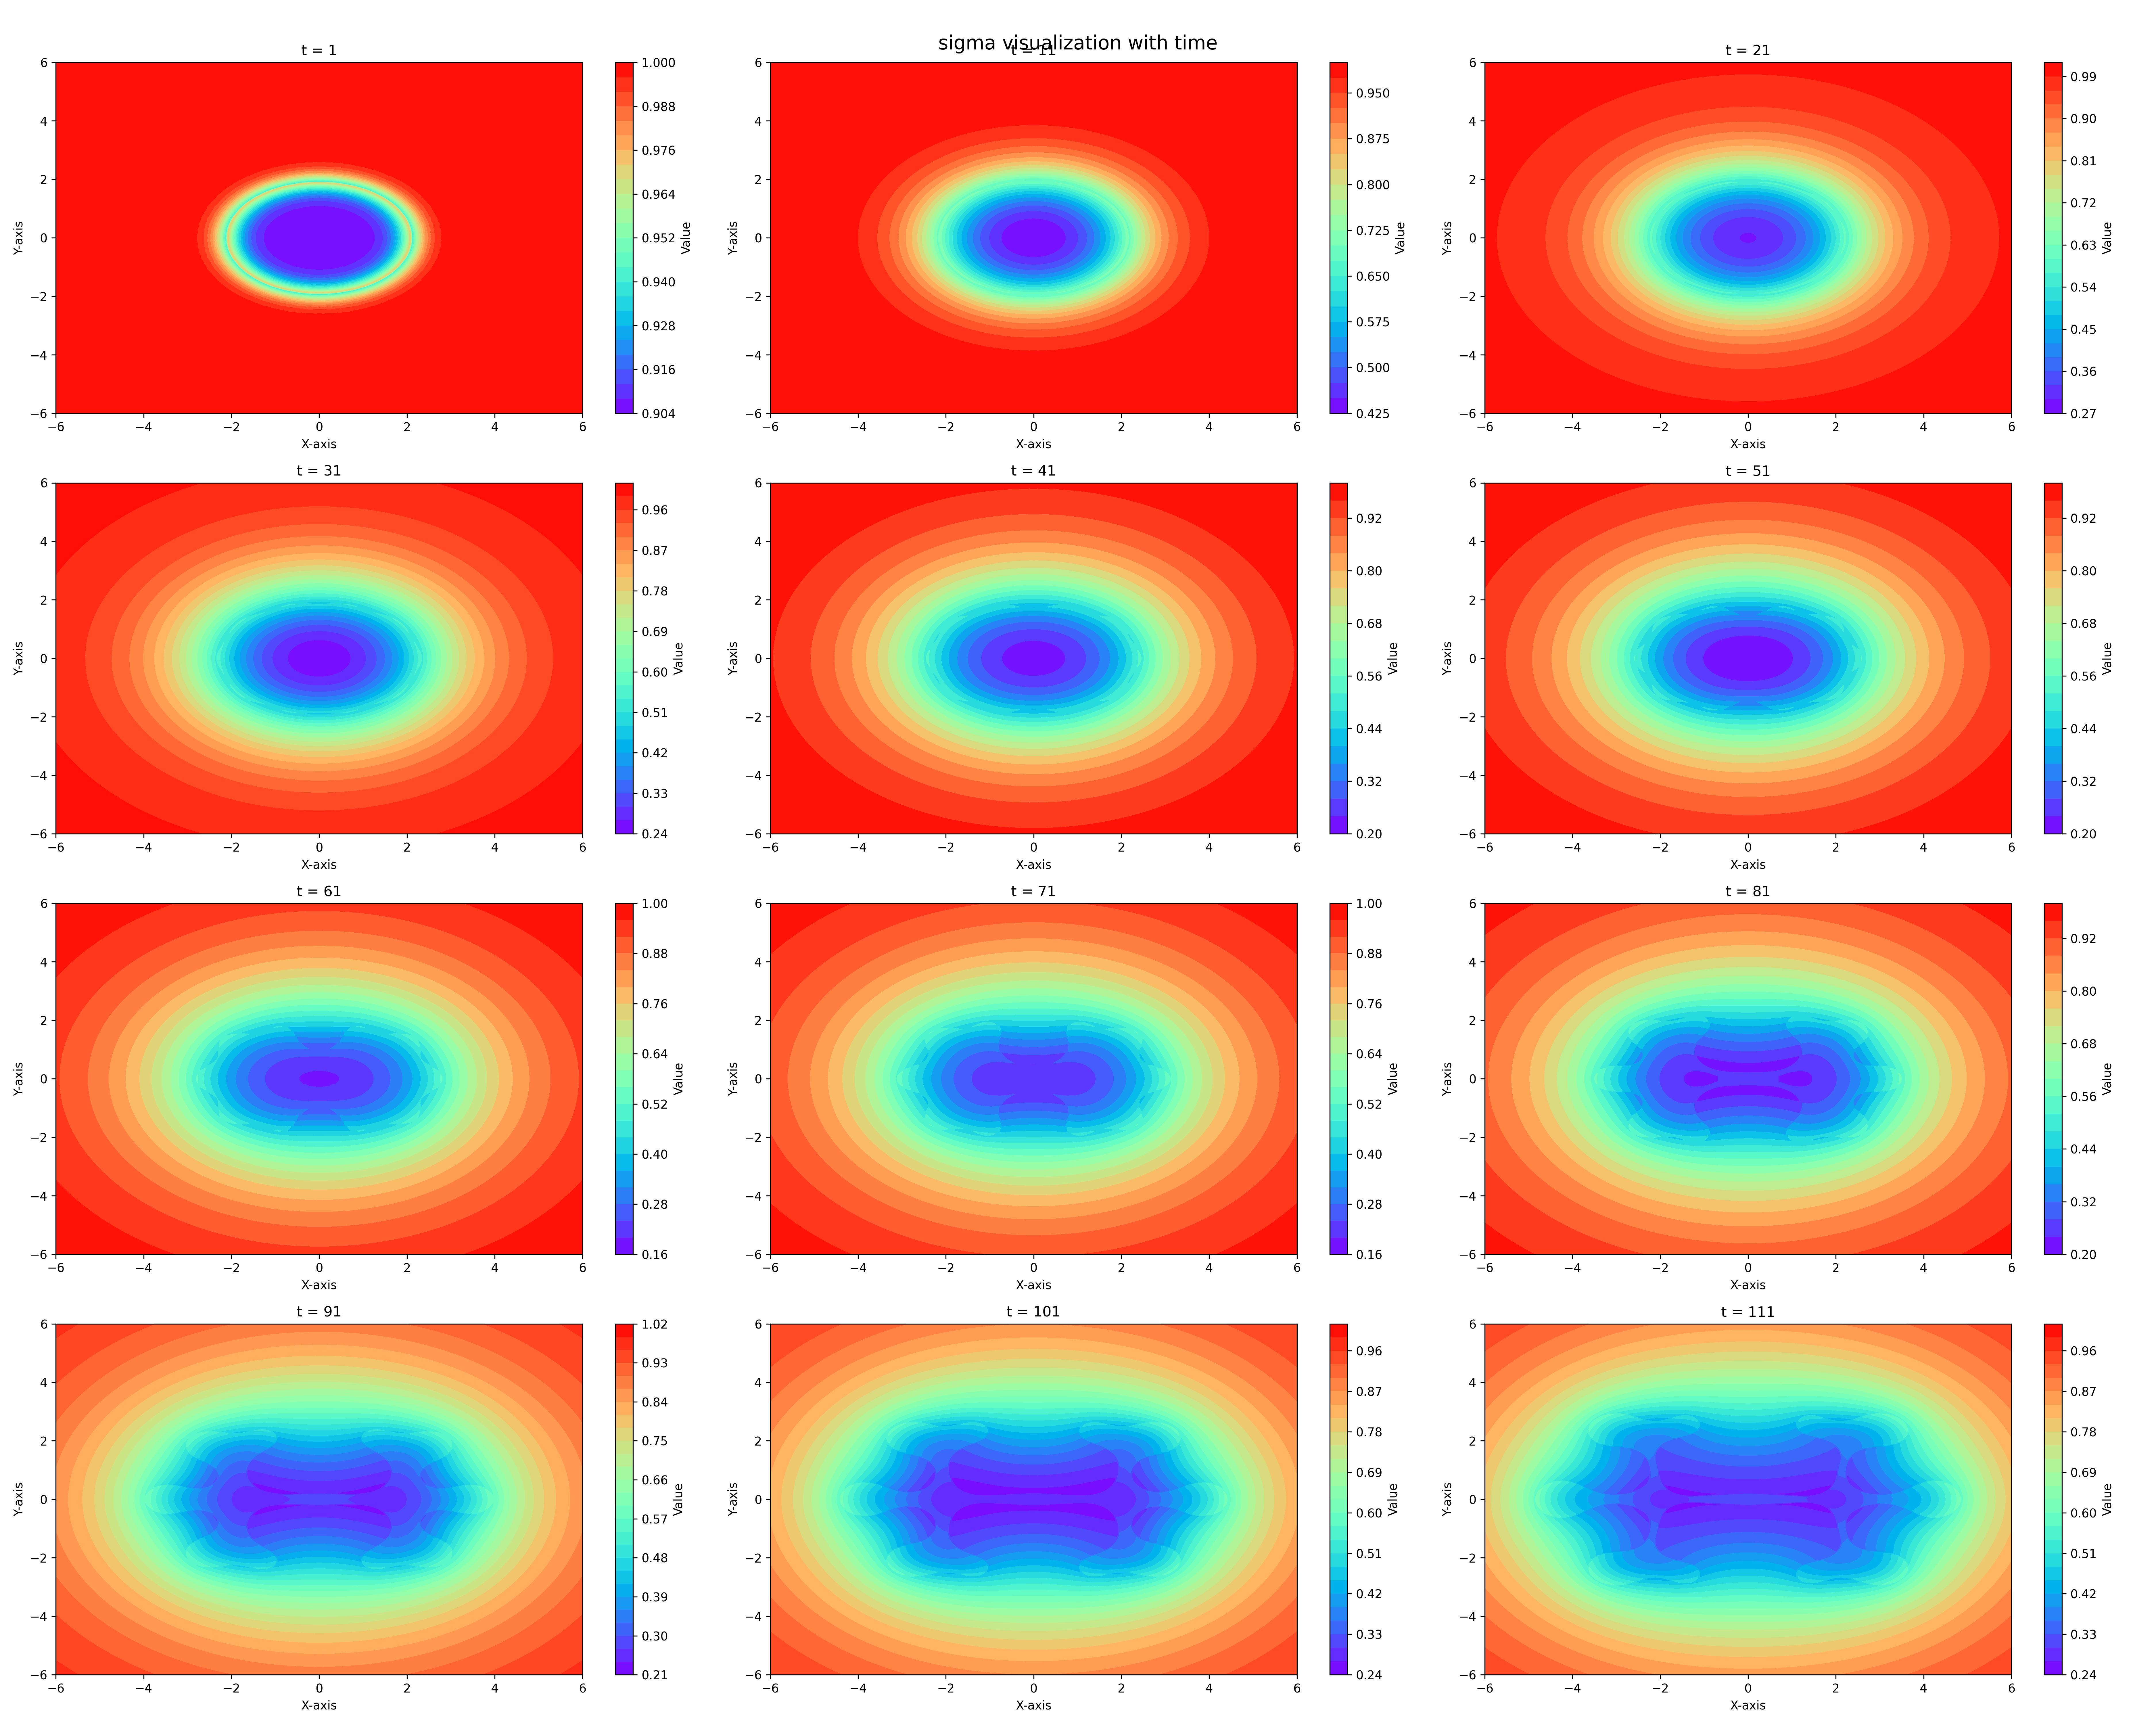
\includegraphics[width=1.0\textwidth]{../sigmaVsT_contour_chi5.png}
    \caption{Contour plot of $\sigma$ with time evolution.}
    \label{fig:sigmaVsT_contour_chi5}
\end{figure*}
Figure \ref{fig:sigmaVsT_scatter_chi10} and \ref{fig:sigmaVsT_contour_chi10} show the evolution of $\sigma$ with time for $\chi_\phi=10$ by plotting the scatter and contour plots respectively. 
Here $t=1$ signifies, 1000 timesteps, with stepsize of 0.001.
\begin{figure*}
    \centering
    \includegraphics[width=1.0\textwidth]{../sigmaVsT_scatter_chi10.png}
    \caption{Scatter plot of $\sigma$ with time evolution.}
    \label{fig:sigmaVsT_scatter_chi10}
\end{figure*}
\begin{figure*}
    \centering
    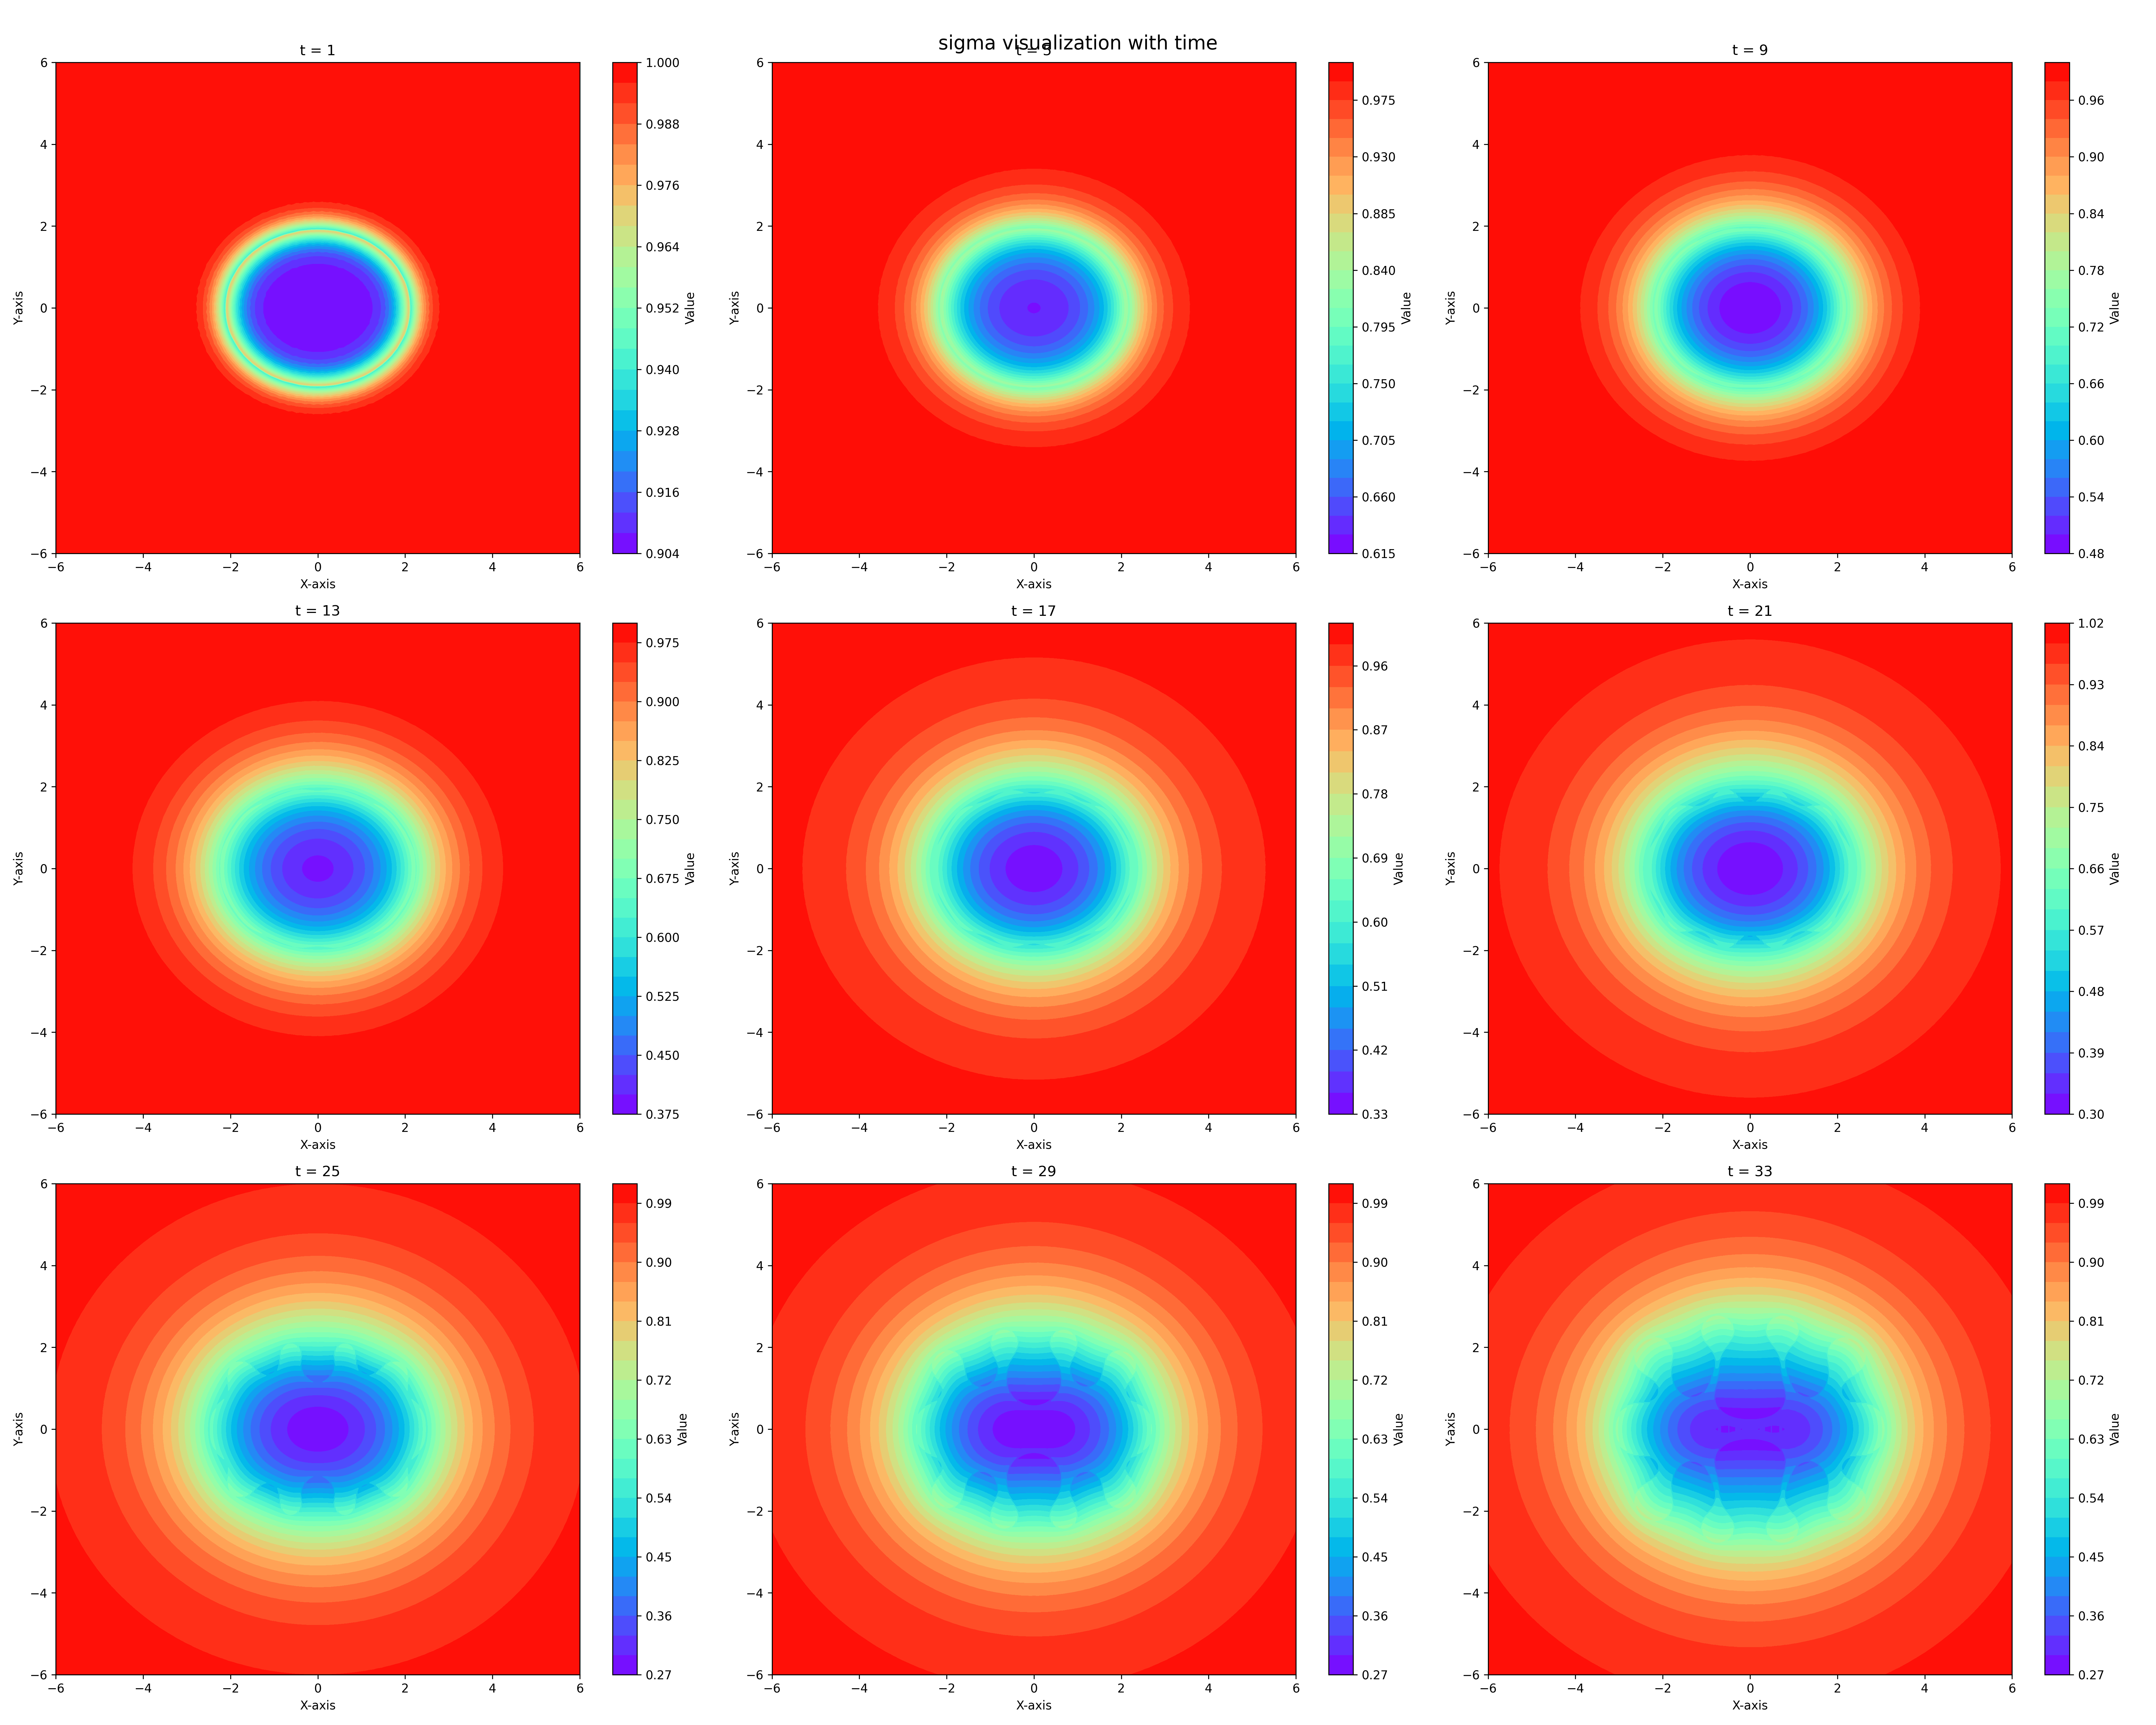
\includegraphics[width=1.0\textwidth]{../sigmaVsT_contour_chi10.png}
    \caption{Contour plot of $\sigma$ with time evolution.}
    \label{fig:sigmaVsT_contour_chi10}
\end{figure*}

\subsection*{$\phi$ Evolution}
Explained by Yoshita Kondapalli in her report.

\section*{Observations}
\begin{itemize}
    \item For larger values of $\chi$ formation and evolution of the branches of tumor is quicker.
    \item More branches are formed in the case of $\chi=10$ as compared to $\chi=5$.
    \item For $\chi=5$, $t=111$ and for $\chi=10$, $t=33$ shows similar evoltion of $\sigma$.
    \item Results are similar to the reference results.
\end{itemize}
Time for execution of the code is around 3-5 seconds per iteration of timestep.
We have ran for $t=150$ i.e., 15000 timesteps with stepsize of 0.001 for $chi=5$ and it took around a day to run the simulation.
We have ran for $t=50$ i.e., 5000 timesteps with stepsize of 0.001 for $chi=10$ and it took around 12 hours to run the simulation.

\section*{Reference Results}
Reference results are obtained from the paper \ref{ref:1}. 
\begin{figure}[h]
    \centering
    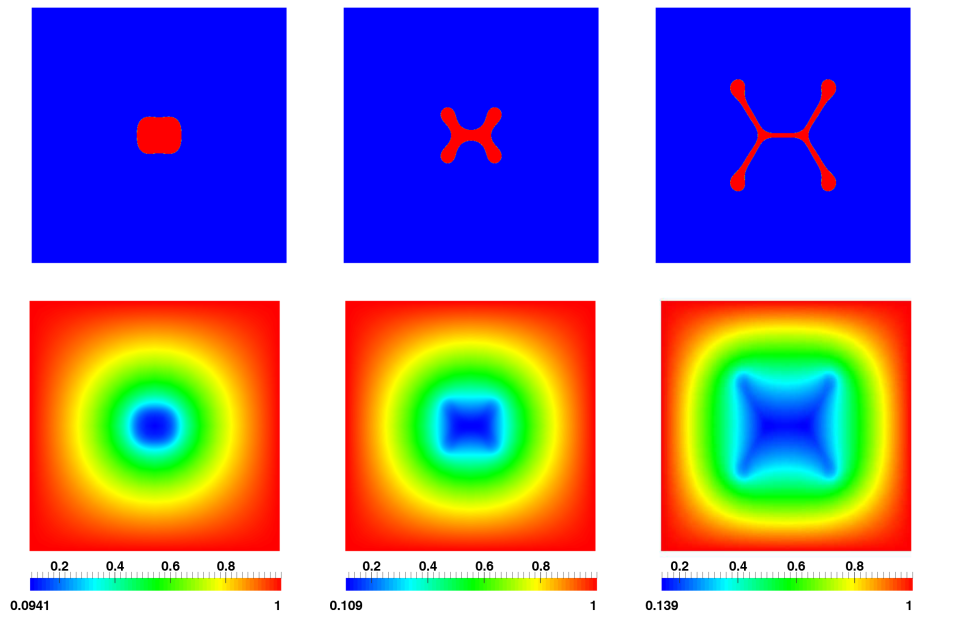
\includegraphics[width=0.8\textwidth]{figures/refRes1.png}
    \caption{Reference Result: Solution with$ P=0.1, \chi_phi=5$, at $t=5, 10, 20$}
    \label{fig:refRes1}
\end{figure}
\begin{figure}[h]
    \centering
    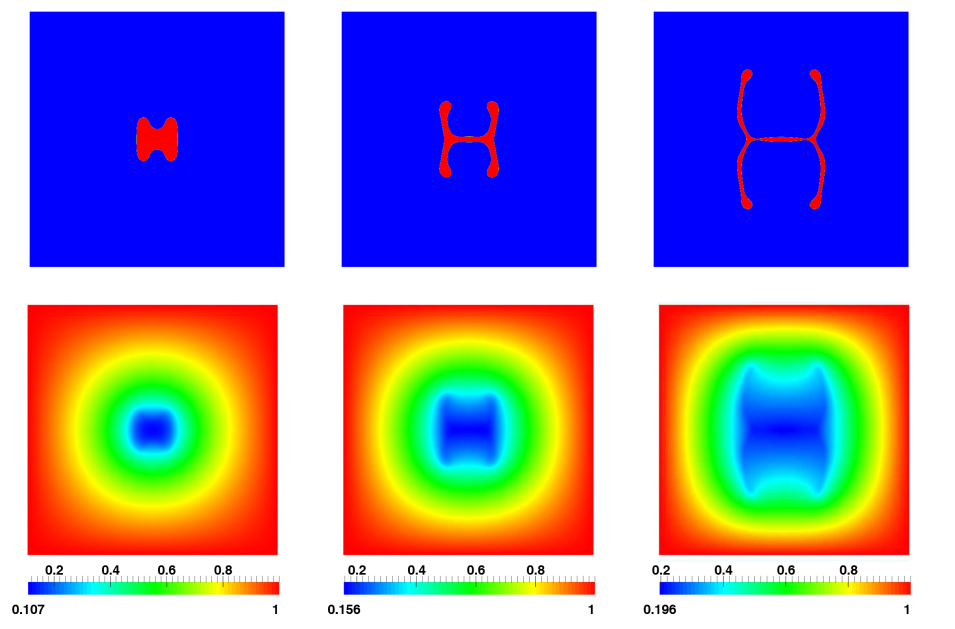
\includegraphics[width=0.8\textwidth]{figures/refRes2.png}
    \caption{Reference Result: Solution with $P=0.1, \chi_{\phi}=10$, at $t=5, 10, 20$}
    \label{fig:refRes2}
\end{figure}
\begin{figure}[h]
    \centering
    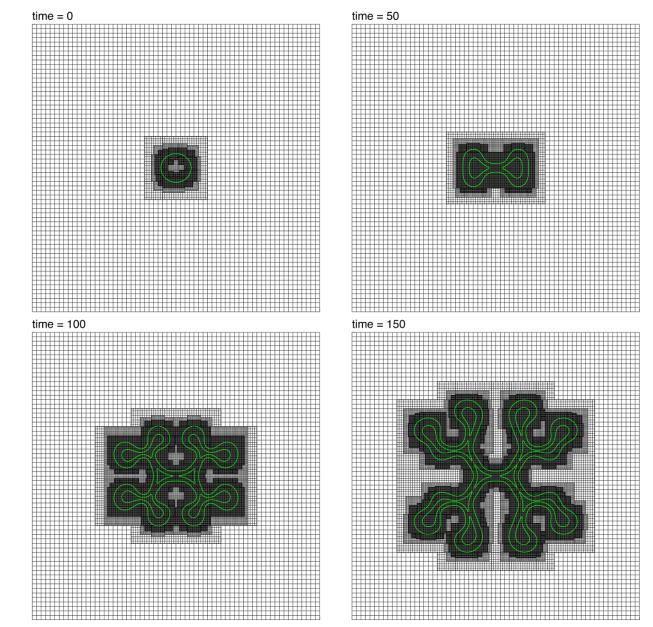
\includegraphics[width=0.8\textwidth]{figures/refRes3.png}
    \caption{Reference Result: From the paper \ref{ref:3}}
    \label{fig:refRes3}
\end{figure}

\section*{Reference}
\begin{enumerate}
    \item \label{ref:1} Garcke, Harald \& Lam, Kei \& Sitka, Emanuel \& Styles, Vanessa. (2016). A Cahn–Hilliard–Darcy model for tumour growth with chemotaxis and active transport. Mathematical Models and Methods in Applied Sciences. 26. 1095-1148. 10.1142/S0218202516500263. 
    \item Non-linear Cahn-Hillard equation using FEM and Newton method. \url{https://docs.fenicsproject.org/dolfinx/main/python/demos/demo_cahn-hilliard.html}
    \item \label{ref:3}Wise, S. M., Lowengrub, J. S., \& Cristini, V. (2011). An adaptive multigrid algorithm for simulating solid tumor growth using mixture models. \textit{Mathematical and Computer Modelling}, 53, 1–20.
\end{enumerate}

\end{document}
